% chapter 3 section 2

\section{声波}

\subsection{声波}
\label{subsec:3.2.1}

\subsubsection{基本信息}

声波日文为音波,其基本内容与第一节相仿,在此仅逐条列举一些基本信息。
\begin{itemize}
    \item 介质:任何物体
    \item 本质:纵波
    \item 频率:20$\sim$20000Hz(人耳感知范围)
    \item 声速:空气中声速随温度改变:$v\approx331.5+0.6t$
    \item 三要素
    \begin{itemize}
        \item 音の高さ:取决于频率$f$
        \item 音色:取决于传递声音的介质
        \item 音の強さ:取决于$f^2A^2$,即日常使用的分贝(db, decibel)
    \end{itemize}
\end{itemize}

\subsubsection{差频}

日文为うなり,是两束频率相近的声波叠加时所发生的相互加强减弱的现象。其叠加而成的声波的频率满足以下公式。
\begin{itembox}[l]{差频公式}
    \begin{equation*}
        f=|f_1-f_2|
    \end{equation*}
\end{itembox}
\begin{figure}[ht!]
    \centering
    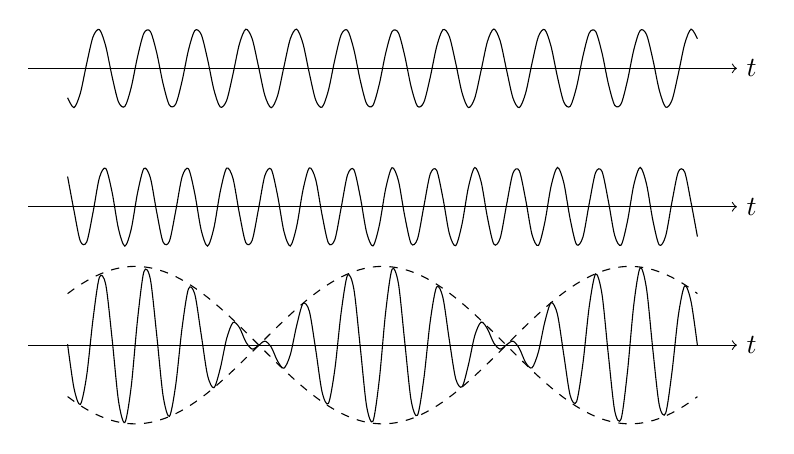
\begin{tikzpicture}
        \begin{scope}[yscale=0.5]
            \draw[->] (-4.5,0) -- (4.5,0) node[right] {$t$};
            \draw[domain=-4:4] plot[samples=100, smooth] (\x, {sin(10*\x r)});
        \end{scope}
        \begin{scope}[yscale=0.5, yshift=-100]
            \draw[->] (-4.5,0) -- (4.5,0) node[right] {$t$};
            \draw[domain=-4:4] plot[samples=100, smooth] (\x, {sin(12*\x r)});
        \end{scope}
        \begin{scope}[yscale=0.5, yshift=-200]
            \draw[->] (-4.5,0) -- (4.5,0) node[right] {$t$};
            \draw[domain=-4:4] plot[samples=100, smooth] (\x, {sin(10*\x r)+sin(12*\x r)});
            \draw[dashed, domain=-4:4] plot[samples=100, smooth] (\x, {2*cos(\x r)});
            \draw[dashed, domain=-4:4] plot[samples=100, smooth] (\x, {-2*cos(\x r)});
        \end{scope}
    \end{tikzpicture}
    \caption{差频}
\end{figure}
实际题目中常与下一小节的多普勒效应结合。

\subsection{多普勒效应}
\label{subsec:3.2.2}

日文为ドップラー効果,是观测者与波源存在相对运动时所发生的观测频率与波源频率不同的现象,日常生活中火车进站、警车鸣笛均属此类。根据观测者与波源的相对运动关系可分为以下三类。

\subsubsection{波源运动,观测者静止}

\begin{figure}[ht!]
    \centering
    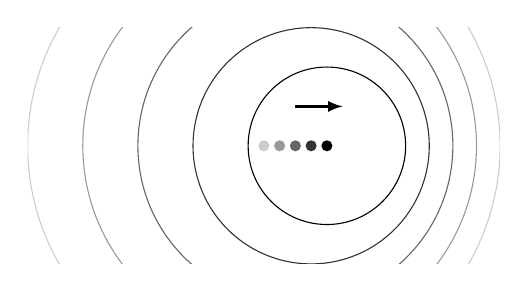
\begin{tikzpicture}
        \clip (-3,-1.5) rectangle (3,1.5);
        \foreach \x/\r in {0/3, 0.2/2.5, 0.4/2, 0.6/1.5, 0.8/1} {
            \fill[opacity={\x+0.2}] (\x,0) circle (2pt);
            \draw[opacity={\x+0.2}] (\x,0) circle (\r);
        }
        \draw[thick, -latex] (0.4,0.5) -- (1,0.5);
    \end{tikzpicture}
    \caption{多普勒效应}
\end{figure}
由图可见,处于波源行进方向上的观测者会遇到更加密集的波面,反之则会遇到更加稀疏的波面。此所谓密集与稀疏实际指的是波面的间距,即波长。因此可以说波源的移动压缩/拉伸了波长。此时以波源为基准观察波速即为$V\pm v$。于是,根据波的基本公式可以得到以下结论。
\begin{equation*}
    V\pm v=f\lambda^\prime\implies
    \lambda^\prime=\frac{V\pm v}{f}
\end{equation*}
在观测者看来波仍然在以原速传播,所以观测者所感知到的频率即为
\begin{equation*}
    f^\prime=\frac{V}{\lambda^\prime}=\frac{V}{V\pm v}f
\end{equation*}

\subsubsection{波源静止,观测者运动}

此时,波源不移动,波长不发生改变。相当于观测者与各个波面在做追及+相遇,倘若两者相向而行,则单位时间内观测者会遇到更多的波面。反之则会遇到更少的波面。根据波的基本公式可以得到以下结论。
\begin{equation*}
    V\pm u=f^\prime\lambda\implies
    f^\prime=\frac{V\pm u}{\lambda}
    =\frac{V\pm u}{V}f
\end{equation*}

\subsubsection{波源运动,观测者运动}

基于上述两种情况的分析,我们可以把双方都运动的问题化简为运动的观测者感知波源压缩/拉伸后的波的问题。
\begin{itembox}[l]{多普勒效应}
    \begin{equation*}
        f^\prime=\frac{V\pm u}{V\pm v}f
    \end{equation*}
    \begin{itemize}
        \item V:波速
        \item u:观测者的速度
        \item v:波源的速度
    \end{itemize}
\end{itembox}
使用上述公式时应注意如下两点:
\begin{itemize}
    \item 观测者的速度和波源的速度的位置
    \item 分数中两个符号的判断\footnote{一般是结合推导过程记忆,但更推荐根据生活经验判断}
\end{itemize}
此外在实际题目中时而也会遇到一些其他变形。比如平面上的多普勒效应\footnote{基于运动的矢量性进行分解,只考虑发生多普勒效应的方向}、含有风的情况\footnote{风会带动介质运动,所以相当于改变了波速}等等。

\subsection{共振现象}
\label{subsec:3.2.3}

\paragraph{共振·共鸣}一般物体都具有一个固定的振动周期,当外界发生与之相同频率的变化时,该物体会受到其影响而发生距离振动的现象。当振动是以声音的形式展现时特称共鸣。

\subsubsection{弦振动}

拨动两端固定的弦,这个振动在弦上会以横波的形式向两端传播,到达端点后发生固定端反射,从而最终在弦上形成驻波。设弦的张力为$S$、线密度为$\rho$,则弦上波速可求。
\begin{figure}[ht!]
    \centering
    \begin{minipage}{0.48\textwidth}
        \begin{itembox}[l]{弦上波速}
            \begin{equation*}
                v=\sqrt{\frac{S}{\rho}}
            \end{equation*}
        \end{itembox}
        \begin{itembox}[l]{弦振动频率}
            \begin{itemize}
                \item $\lambda=\frac{2}{n}l$
                \item $f=\frac{nv}{2l}\implies nf_1=f_n$
            \end{itemize}
        \end{itembox}
    \end{minipage}
    \begin{minipage}{0.48\textwidth}
        \centering
        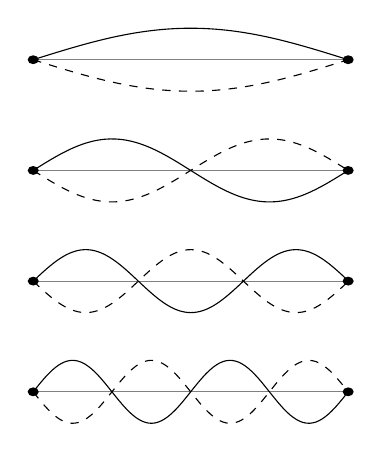
\begin{tikzpicture}
            \foreach \t/\yshift in {
                8/0, 4/-50, 2.67/-100, 2/-150
            } {
                \begin{scope}[yscale=0.8, yshift=\yshift]
                    \draw[color=gray] (0,0) -- (4,0);
                    \fill (0,0) circle (2pt);
                    \fill (4,0) circle (2pt);
                    \draw[domain=0:4] plot[samples=50, smooth] (\x, {0.5*sin((2*pi/\t)*(\x r)});
                    \draw[dashed, domain=0:4] plot[samples=50, smooth] (\x, {-0.5*sin((2*pi/\t)*(\x r)});
                \end{scope}
            }
        \end{tikzpicture}
        \caption{弦振动}
    \end{minipage}
\end{figure}
此外可以稳定形成驻波的振动均为弦的固有振动,其中我们将只有一个波峰的振动形式称为基本振动,称频率为基本振动频率n倍的振动形式为n倍振动。

\subsubsection{气柱振动}

与弦振动类似,通过吹气等方式使管内空气发生振动,同样也能形成驻波。当管口封闭时该端点形成固定端,反之形成自由端。我们将两端均开口的管称为开管,将一端开口、一端闭口的管称为闭管。分析其振动规律可得气柱振动的波长、频率等信息。此外对于闭管振动会出现开口端腹点(加强点)外移的现象\footnote{开口端补正:固定频率,改变管长,可由两次共振时的管长求得次偏移值。$\Delta x=\frac{l_2-3l_1}{2}$},但考试中鲜有提及,故此处略过。
\begin{figure}[ht!]
    \centering
    \begin{minipage}[t]{0.48\textwidth}
        \centering
        \begin{tikzpicture}
            \foreach \n/\t/\yshift in {
                1/8/0, 2/4/-50, 3/2.67/-100, 4/2/-150
            } {
                \begin{scope}[yscale=0.6, yshift=\yshift]
                    \node at (-1,0) {\n 倍振动};
                    \fill[fill=gray, opacity=0.2] (0,-0.6) rectangle (4,0.6);
                    \draw[thick] (0,0.6) -- (4,0.6);
                    \draw[thick] (0,-0.6) -- (4,-0.6);
                    \draw[domain=0:4] plot[samples=50, smooth] (\x, {0.5*cos((2*pi/\t)*(\x r)});
                    \draw[dashed, domain=0:4] plot[samples=50, smooth] (\x, {-0.5*cos((2*pi/\t)*(\x r)});
                \end{scope}
            }
        \end{tikzpicture}
        \caption{开管振动}
    \end{minipage}
    \begin{minipage}[t]{0.48\textwidth}
        \centering
        \begin{tikzpicture}
            \foreach \n/\t/\yshift in {
                1/16/0, 3/5.33/-50, 5/3.2/-100, 7/2.29/-150
            } {
                \begin{scope}[yscale=0.6, yshift=\yshift]
                    \node at (-1,0) {\n 倍振动};
                    \fill[fill=gray, opacity=0.2] (0,-0.6) rectangle (4,0.6);
                    \draw[thick] (4,-0.6) -- (0,-0.6) -- (0,0.6) -- (4,0.6);
                    \draw[domain=0:4] plot[samples=50, smooth] (\x, {0.5*sin((2*pi/\t)*(\x r)});
                    \draw[dashed, domain=0:4] plot[samples=50, smooth] (\x, {-0.5*sin((2*pi/\t)*(\x r)});
                \end{scope}
            }
        \end{tikzpicture}
        \caption{闭管振动}
    \end{minipage}
\end{figure}
\begin{itembox}[l]{气柱振动}
    \begin{itemize}
        \item 开管振动
        \begin{itemize}
            \item $\lambda=\frac{2}{n}l$
            \item $f=\frac{nv}{2l}\implies nf_1=f_n$
        \end{itemize}
        \item 闭管振动
        \begin{itemize}
            \item $\lambda=\frac{4}{2n-1}l$
            \item $f=\frac{(2n-1)v}{4l}\implies (2n-1)f_1=f_n$
        \end{itemize}
    \end{itemize}
\end{itembox}
